\documentclass[a4paper,12pt]{scrartcl}  %% article, see KOMA 
\usepackage[english]{babel}
\usepackage{caption}
\captionsetup[figure]{labelfont={color=blue}}
\usepackage{color}
\usepackage[usenames,dvipsnames,svgnames,table]{xcolor}
\usepackage[backref=true,backend=bibtex,natbib=true,hyperref=true, 
style=numeric, sorting=none]{biblatex}

\addbibresource{../bibliography.bib}
\renewcommand{\labelnamepunct}{\addcolon\space} % Doppelpunkt anstatt des Punkts nach dem Autor und vor dem Titel der Arbeit
\usepackage[T1]{fontenc}
\usepackage[utf8]{inputenc}
\usepackage{lmodern}
\usepackage{ae,aecompl}
\usepackage{amsmath}
\usepackage{amsfonts}
\usepackage{amssymb}
\usepackage{psfrag}
\usepackage{authblk}
\usepackage{physics}
\usepackage{mathtools}
\usepackage{bm}
\usepackage{tikz}
\definecolor{rgray1}{gray}{0.85}
\definecolor{rgray2}{gray}{0.9}
\definecolor{rgray3}{gray}{0.95}

\renewcommand*\sectfont{\normalcolor\rmfamily\bfseries}
\renewcommand*\descfont{\rmfamily\bfseries}

%%% listings: include programming code
%\usepackage{listings}

%%% units: technical units
%\usepackage{units}
\usepackage[automark]{scrpage2}
\usepackage{ifpdf}

\ifpdf
  %%% graphicx: support for graphics
  %\usepackage[pdftex]{graphicx}
  \usepackage[pdftex=true,backref,pagebackref=false,colorlinks=true,
    bookmarks=true, bookmarksopen=false, bookmarksnumbered=false,
    pdfpagemode=None]{hyperref}
  \hypersetup{linkcolor = RoyalBlue, citecolor = RoyalBlue, urlcolor=WildStrawberry}
  \usepackage{cleveref}
  \DeclareGraphicsExtensions{.pdf}
\else
\usepackage[dvips]{graphicx}

  \DeclareGraphicsExtensions{.eps}

  \usepackage[dvips]{hyperref}
\fi

\hypersetup{
  pdftitle={Design of a broadband metamaterial absorber for the X-band}, %%
  pdfauthor={Dr. Stefan Umrath}, %%
  pdfsubject={}, %%
  pdfcreator={LaTeX with hyperref-package.}, %% 
  pdfproducer={}, %%
  pdfkeywords={} %%
}

\newcommand{\mygraphics}[3]{
  \begin{center}
    \includegraphics[width=#1, keepaspectratio=true]{#2} \\
    \textbf{#3}
  \end{center}
}
\renewcommand{\Cref}[1]{\cref{#1}\textcolor{RoyalBlue}{)}}
\newcommand{\capFref}[1]{Fig. \ref{#1}\textcolor{RoyalBlue}{)}}
\newcommand{\capEref}[1]{Eq. \textcolor{RoyalBlue}{(}\ref{#1}\textcolor{RoyalBlue}{)}}
\newcommand{\Ref}[1]{\ref{#1}\textcolor{RoyalBlue}{)}}
\newcommand{\unitv}[1]{\hat{\bm{#1}}}
\newcommand{\imag}{\mathrm{i}}
\newcommand{\euler}{\mathrm{e}}
\renewcommand{\dyad}[1]{\overset{\bm\leftrightarrow}{#1}}
\newcommand{\rd}{\mathrm{d}}
%\newcommand{\ontop}{\genfrac{\{}{\}}{0pt}{}}
\newcommand\ontop[4]{\genfrac{#1}{#2}{0pt}{}{#3}{#4}}


\title{Metamaterial Absorbers}

%%% author(s)
\author[1]{Dr. Stefan Umrath, \href{mailto:Stefan.Umrath@dlr.de}{Stefan.Umrath@dlr.de}}
\affil[1]{German Aerospace Center (DLR)}
\date{Oberpfaffenhofen \today{} \vspace{3cm}}
\bibliography{bibliography.bib}



\begin{document}

\maketitle
\begin{center}

\includegraphics[width= 0.75\linewidth]{../media/DLR_Logo_engl_schwarz.jpg}
\end{center}

\newpage
\tableofcontents 
\newpage
\section{Motivation}
%Die Verwendung von elektromagnetischen Wellen hat mit der voranschreitenden 
%Digitalisierung und Vernetzung stark zugenommen. Damit hat einerseits die 
%Optimierung der Abstrahl-/Emfangseigenschaften von Sendern bzw. Emfängern 
%an Wichtigkeit gewonnen und andererseits die Detektion von passiven, d. h. 
%weder sendenden, noch empfangenden. Als Beispiele seinen die Mobilfunkkommunikation, 
%autonom navigierende Fahrzeuge, oder die Luftraumüberwachung genannt, welche
%sich u. a. mit der Detektion von Drohnen und feindlichen Flugzeugen beschäftigt. 
%In all diesen Bereichen gibt es Anwendungen für Materialien, welche von 
%Menschenhand mit einer speziellen Wirkung auf elektromagnetische Wellen
%ausgestattet wurden, sog. Metamaterialien.

Metamaterials are man-made artificial materials with electromagnetical properties which
tailored to enable them to manipulate light or radar waves in a desired way.
Their design has become possible due to the computational power of todays computing systems on the one hand
and approriate methods for manufacturing submilimeter conducting structures. Todays research in the field of
metamaterials includes the design of flat, cheap and lightweight microwave absorbers, cloaks, radomes 
with enhanced transmission properties and devices which can harvest the energy of the sun more 
effectively than their conventional counterparts.

In case of microwave or radar absorbing materials (RAM) the callenge is to design structures
which exhibit either absorption of incoming radiation at sharply defined frequncies or obtain broadband
absorption characteristics. 
Due to mutual interaction of resonant metallic inclusions in a unitcell obtaining absorption at two or more 
frequencies is not an easy task. \capFref{fig:Wifi} depicts a 3x3 array of a unitcell which conists of two concentric conducting rings placed on a dielectric FR4 subsrtate. Due to its high degree of symmetry the reflection response of this structure is not only independent of the polarization of incoming radition but 
the freedom to choose the radii of the rings allows for adjusting the absorption frequencies.
When it comes to broadband microwave absorbers, mechanisms must be found, which interconnect multiple neighboring absorption peaks to obtain absorption over an interval of frequencies. \capFref{fig:XBand} shows 
a unitcell with broadband reflection attenuation. The key idea of turning the unitcell to a broadband absorber is the introduction of loss by means of surface mount resistors (shown in black).

\section{Metamaterialien für Reflexionsdämpfung}
Überall dort, wo Reflexion von elektromagnetischen Wellen unterdrückt werden sollen
und spezielle Anforderungen an das Absorbermaterial gestellt werden, können 
Metamaterialabsorber eingesetzt werden. 
Entsprechend des Einsatzgebiets können Metamaterialabsorber ihren konventionellen
Absorbern auf Basis von magnetischen Materialien oder Schaumabsorbern in Punkto Gewicht, Dicke, Herstellungspreis überlegen sein. Je nach Anwendungszweck können Absorber mit
Wirksamkeit über einen breiten Frequenzbereich oder schmalbandig erwünscht sein. 
Um die Machbarkeit für beide Szenarien zu demonsiereren, wurden ein schmalbandiger Absorber für zwei weit verbreitete WLan-Frequnezen, sowie ein Breitbandabsorber für das militärisch relevante X-Band entwickelt, simuliert, gefertigt und vermessen.

\begin{figure}
\centering
\begin{minipage}[b]{0.5\textwidth}
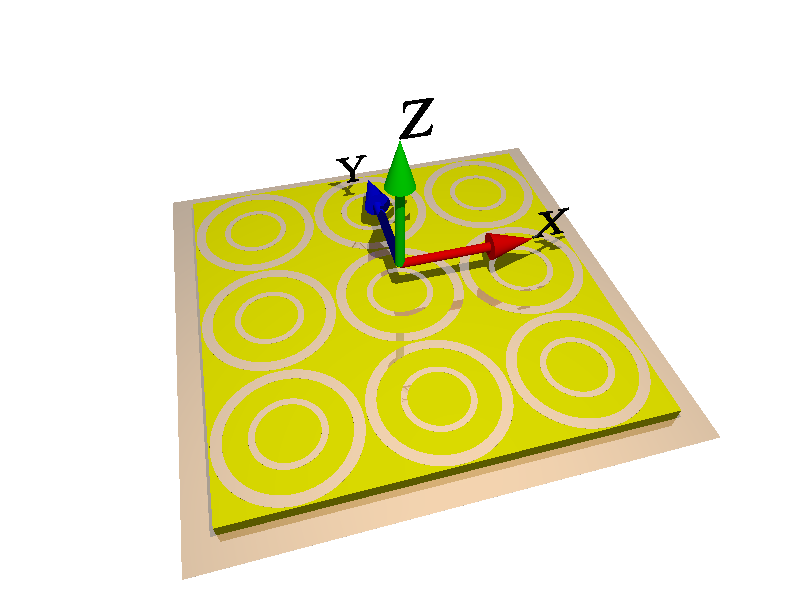
\includegraphics[scale=0.3]{../media/double_rings.png}
\caption{Unitcell for a metamaterial absorber working at the WiFi frequencies 2.4 and 5.2 GHz.}
\label{fig:Wifi}
\hspace{55pt}
\end{minipage}
\begin{minipage}[b]{0.4\textwidth}
\includegraphics[scale=0.3]{../media/XBandAbsorber.png}
\caption{Unitcell for a metamaterial absorber desigend for the X-Band.}
\label{fig:XBand}
\end{minipage}
\end{figure}




\newpage


%%% name of the bibliography file without .bib
%%% e.g.: literatur.bib -> 

\printbibliography


\end{document}
